\ifx\wholebook\relax\else
\documentclass[twoside]{book}
\usepackage[active]{srcltx}
\usepackage[LY1]{fontenc}
\usepackage{epsfig}
\def\etc{{\it etc}}
\def\eg{{\it e.g.}}
\def\ie{{\it i.e.}}
\def\cf{{\it c.f.}\ }
\def\erf{\mathop{\rm erf}}
\def\sign{\mathop{\rm sign}}
\def\prob{\mathop{\rm Prob}}
\def\var{\mathop{\rm var}}
\def\mod{\mathop{\rm mod}}
\def\cor{\mathop{\rm cor}}
\def\cov{\mathop{\rm cov}}
\def\cl{\mathop{\rm CL}}
\def\kg{\mathop{\rm Kg}}
\def\patstyle#1{{\sc #1}}
\def\th{^{\mathop{\rm th}}}
\def\st#1{^{\mathop{\rm #1}}}
\def\note#1{\begin{quote}{\bf Note:} #1\end{quote}}
\def\braket#1{\left\langle #1\right\rangle}
\def\order#1{\let\o=#1{\cal O}\ifx\o 1$\left(n\right)$\else$\left(n^{#1}\right)$\fi}
\newtheorem{privListing}{Listing}[chapter]
\newenvironment{listing}{\vskip 3ex\hrule\vskip 1ex\begin{privListing}}{\end{privListing}\hrule\vskip 1ex}
\newtheorem{privExample}{Code example}[chapter]
\newenvironment{codeExample}{\begin{privExample}\begin{quote}\tt}{\end{quote}\end{privExample}}
\def\relboxl#1#2{\hbox to #1\hsize{#2\hfil}}
\def\relboxc#1#2{\hbox to #1\hsize{\hfil #2\hfil}}
\def\relboxr#1#2{\hbox to #1\hsize{\hfil #2}}
\def\transpose#1{{\bf #1}^{\mathop{\rm T}}}
\def\inverse#1{{\bf #1}^{-1}}
%\def\tm{$^{\mathop{\rm TM}}$}
\def\tm{ }
\newenvironment{mainEquation}{\marginpar[\vspace{3 ex} Main
equation$\Rightarrow$]{\vspace{3 ex}$\Leftarrow$Main
equation}\begin{equation}}{\end{equation}}
\def\rubrique#1{\paragraph{#1}\hfil\par\noindent}

\begin{document}
\fi

\chapter{Introduction} \vspace{1 ex}
\label{ch:introduction}
\begin{flushright}
{\sl Science sans conscience n'est que ruine de
l'\^ame.}\footnote{Science without consciousness just ruins the
soul.}\\ Fran\c{c}ois Rabelais
\end{flushright}
\vspace{1 ex} Teaching numerical methods was a major discipline of
computer science at a time computers were only used by a very
small amount of professionals such as physicists or operation
research technicians. At that time most of the problems solved
with the help of a computer were of numerical nature, such as
matrix inversion or optimization of a function with many
parameters.
\par
With the advent of minicomputers, workstations and foremost,
personal computers, the scope of problems solved with a computer
shifted from the realm of numerical analysis to that of symbol
manipulation. Recently, the main use of a computer has been
centered on office automation. Major applications are word
processors and database applications.
\par
Today, computers are no longer working stand-alone. Instead they
are sharing information with other computers. Large databases are
getting commonplace. The wealth of information stored in large
databases tends to be ignored, mainly because only few persons
knows how to get access to it and an even fewer number know how to
extract useful information. Recently people have started to tackle
this problem under the buzzword data mining. In truth, data mining
is nothing else than good old numerical data analysis performed by
high-energy physicists with the help of computers. Of course a few
new techniques are been invented recently, but most of the field
now consists of rediscovering algorithms used in the past. This
past goes back to the day Enrico Fermi used the ENIAC to perform
phase shift analysis to determine the nature of nuclear forces.
\par
The interesting point, however, is that, with the advent of data
mining, numerical methods are back on the scene of information
technologies.

\section{Object-oriented paradigm and mathematical objects}
In recent years object-oriented programming (OOP) has been welcomed for its
ability to represent objects from the real world (employees, bank accounts,
etc.) inside a computer.
Herein resides the formidable leverage of object-oriented
programming.
It turns out that this way of looking at OOP is somewhat overstated (as these
lines are written).
Objects manipulated inside an object-oriented program certainly do not
behave like their real world counterparts. Computer objects are
only models of those of the real world. The Unified Modeling Language (UML) user
guide goes further in stating that {\it a model is a simplification of
reality} and we should emphasize that it is {\sl only that}. OOP
modeling is so powerful, however, that people tend to forget about
it and only think in terms of real-world objects.
\par
An area where the behavior of computer objects nearly reproduces
that of their real-world counterparts is mathematics. Mathematical
objects are organized within {\it hierarchies}. For example,
natural integers are included in integers (signed integers), which
are included in rational numbers, themselves included in real
numbers. Mathematical objects use {\it polymorphism} in that one
operation can be defined on several entities. For example,
addition and multiplication are defined for numbers, vectors,
matrices, polynomials --- as we shall see in this book --- and
many other mathematical entities. Common properties can be
established as an abstract concept (\eg a group) without the
need to specify a concrete implementation. Such concepts can then
be used to prove a given property for a concrete case. All this
looks very similar to {\sl class hierarchies}, {\sl methods} and
{\sl inheritance}.
\par
Because of these similarities OOP offers the possibility to
manipulate mathematical objects in such a way that the boundary
between real objects and their computer models becomes almost
non-existent. This is no surprise since the structure of OOP
objects is equivalent to that of mathematical
objects\footnote{From the point of view of computer science, OOP
objects are considered as mathematical objects.}. In numerical evaluations,
the equivalence between mathematical
objects and computer objects is almost perfect. One notable
difference remains, however -- namely the finite size of the
representation for noninteger number in a computer limiting the
attainable precision. We shall address this important topic in
section \ref{sec-rounding}.
\par
Most numerical algorithms have been invented long before the widespread use of computers. Algorithms were designed to speed up
human computation and therefore were constructed to minimize
the number of operations to be carried out by the human operator.
Minimizing the number of operations is the best thing to do to
speed up code execution.
\par
One of the most heralded benefits of object-oriented programming
is code reuse, a consequence, in principle, of the hierarchical
structure and of inheritance. The last statement is pondered by
"in principle" since, to date, code reuse of real world objects is
still far from being commonplace.
\par
For all these reasons, this book tries to convince you that using
object-oriented programming for numerical evaluations can exploit
the mathematical definitions to maximize code reuse between many
different algorithms. Such a high degree of reuse yields very
concise code. Not surprisingly, this code is quite efficient and,
most importantly, highly maintainable. Better than an
argumentation, we show how to implement some numerical algorithms
selected among those that, in my opinion, are most useful for the areas
where object-oriented software is used primarily: finance,
medicine and decision support.

\section{Object-oriented concepts in a nutshell}
First let us define what is covered by the adjective {\it
object-oriented}. Many software vendors are qualifying a piece of
software object-oriented as soon as it contains things called
objects, even though the behavior of those objects has little to
do with object-orientation. For many programmers and most software
journalists any software system offering a user interface design
tool on which elements can be pasted on a window and linked to
some events --- even though most of these events are being
restricted to user interactions --- can be called object-oriented.
There are several typical examples of such software, all of them
having the prefix {\it Visual} in their names\footnote{This is not
to say that all products bearing a name with the prefix {\it
Visual} are not object-oriented.}. Visual programming is something
entirely different from object-oriented programming.
\par
Object-oriented is not intrinsically linked
with the user interface. Recently, object-oriented techniques
applied to user interfaces have been widely exposed to the public,
hence the confusion. Three properties are considered
essential for object-oriented software:
\begin{enumerate}
\item data encapsulation,
\item class hierarchy and inheritance,
\item polymorphism.
\end{enumerate}
{\it Data encapsulation} is the fact that each object hides its
internal structure from the rest of the system. Data encapsulation
is in fact a misnomer since an object usually chooses to expose
some of its data. I prefer to use the expression {\it hiding the
implementation}, a more precise description of what is usually
understood by data encapsulation. Hiding the implementation is a
crucial point because an object, once fully tested, is guaranteed
to work ever after. It ensures an easy maintainability of
applications because the internal implementation of an object can
be modified without impacting the application, as long as the
public methods are kept identical.
\par
{\it Class hierarchy and inheritance} is the keystone
implementation of any object-oriented system. {\it A class} is a
description of all properties of all objects of the same type.
These properties can be structural (static) or behavioral
(dynamic). Static properties are mostly described with instance
variables. Dynamic properties are described by methods.
Inheritance is the ability to derive the properties of an object
from those of another. The class of the object from which another
object is deriving its properties is called the superclass. A
powerful technique offered by class hierarchy and inheritance is
the overloading of some of the behavior of the superclass.
\par
{\it Polymorphism} is the ability to manipulate objects from
different classes, not necessarily related by inheritance, through
a common set of methods. To take an example from this book,
polynomials can have the same behavior than signed integers with
respect to arithmetic operations: addition, subtraction,
multiplication and division.
\par
Most so-called object-oriented development tools (as opposed to
languages) usually fail the inheritance and polymorphism
requirements.
\par
The code implementation of the algorithms presented in this book
is given in Smalltalk, one of the best object-oriented programming language.
For this book, we are using Pharo\footnote{http://www.pharo.org/}, a modern
open-source implementation of Smalltalk.

%Both languages are excellent object-oriented languages. I would strongly
%recommend people reading this book to consult the implementation sections of both languages regardless of their personal taste of language. First, I have
%made some effort to use of the best feature of each language. Second, each
%implementation has been made independently. The fact that the code of each
%implementation is different shows that there is indeed many ways to skin a cat,
%even when written by the same person. Thus, looking seriously at both
%implementations can be quite instructive for someone who wants to progress with the object-oriented paradigm.

\section{Dealing with numerical data}
The numerical methods exposed in this book are all applicable to
real numbers. As noted earlier the finite representation of
numbers within a computer limits the precision of numerical
results, thereby causing a departure from the ideal world of
mathematics. This section discusses issues related to this
limitation.

\subsection{Floating point representation}
Currently mankind is using the decimal system\footnote{This is of
course quite fortuitous. Some civilizations have opted for a
different base. The Sumerians have used the base 60 and this habit
has survived until now in our time units. The Maya civilization
was using the base 20. The reader interested in the history of
numbers ought to read the book of Georges Ifrah \cite{Ifrah}.}. In
this system, however, most rational numbers and all irrational and
transcendental numbers escape our way of representation. Numbers
such as 1/3 or $\pi$ cannot be written in the decimal system other
than approximately. One can chose to add more digits to the right
of the decimal point to increase the precision of the
representation. The true value of the number, however, cannot be
represented. Thus, in general, a real number cannot be represented
by a finite decimal representation. This kind of limitation has
nothing to do with the use of computers. To go around that
limitation, mathematicians have invented abstract representations
of numbers, which can be manipulated in regular computations. This
includes irreducible fractions (1/3 \eg), irrational numbers
($\sqrt{2}$ \eg), transcendental numbers ( $\pi$ and $e$ the base
of natural logarithms \eg) and normal\footnote{Since Cantor,
mathematicians have learned that there are many kinds of
infinities. See for example reference \cite{Gullberg}.} infinities
( $-\infty$ and $+\infty$).
\par
Like humans, computers are using a representation with a finite
number of digits, but the digits are restricted to 0 and 1.
Otherwise number representation in a computer can be compared to
the way we represent numbers in writing. Compared to humans
computers have the notable difference that the number of digits
used to represent a number cannot be adjusted during a
computation. There is no such thing as adding a few more decimal
digits to increase precision. One should note that this is only an
implementation choice. One could think of designing a computer
manipulating numbers with adjustable precision. Of course, some
protection should be built in to prevent a number, such as 1/3, to
expand {\it ad infinitum}. Probably, such a computer would be much
slower. Using digital representation --- the word digital being
taken in its first sense, that is, a representation with digits
--- no matter how clever the implementation\footnote{Symbolic
manipulation programs do represent numbers as we do in
mathematics. Such programs are not yet suited for quick numerical
computation, but research in this area is still open.}, most
numbers will always escape the possibility of exact
representation.
\par
In present day computers, a floating-point number is represented
as $m\times r^e$ where the radix $r$ is a fixed number, generally
2. On some machines, however, the radix can be 10 or 16. Thus,
each floating-point number is represented in two
parts\footnote{This is admittedly a simplification. In practice
exponents of floating point numbers are offset to allow negative
exponents. This does not change the point being made in this
section, however.}: an integral part called the mantissa $m$ and
an exponent $e$. This way of doing is quite familiar to people
using large quantities (astronomers \eg) or studying the
microscopic world (microbiologists \eg). Of course, the natural
radix for people is 10. For example, the average distance from
earth to sun expressed in kilometer is written as
$1.4959787\times10^8$.

In the case of radix 2, the number 18446744073709551616 is
represented as $1\times2^{64}$. Quite a short hand compared to the
decimal notation! IEEE standard floating-point numbers use 24 bits
for the mantissa (about 8 decimal digits) in single precision;
they use 53 bits (about 15 decimal digits) in double precision.
\par
One important property of floating-point number representation is
that the relative precision of the representation --- that is the
ratio between the precision and the number itself --- is the same
for all numbers except, of course, for the number 0.

\subsection{Rounding errors}
\label{sec-rounding} To investigate the problem of rounding let us
use our own decimal system limiting ourselves to 15 digits and an
exponent. In this system, the number $2^{64}$ is now written as
$184467440737095\times10^5$. Let us now perform some elementary
arithmetic operations.
\par
First of all, many people are aware of problems occurring with
addition or subtraction. Indeed we have: $$184467440737095\times
10^5+300 = 184467440737095\times 10^5.$$ More generally, adding or
subtracting to $2^{64}$ any number smaller than 100000 is simply
ignored by our representation. This is called a rounding error.
This kind of rounding errors have the non-trivial consequence of
breaking the associative law of addition. For example, $$\left(1
\times 2^{64}+1 \times 2^{16}\right)+1 \times
2^{32}=184467440780044\times10^5,$$ whereas $$1 \times
2^{64}+\left(1 \times 2^{16}+1 \times
2^{32}\right)=184467440780045\times10^5.$$ In the two last
expressions, the operation within the parentheses is performed
first and rounded to the precision of our representation, as this
is done within the floating point arithmetic unit of a
microprocessor\footnote{In modern days microprocessor, a floating
point arithmetic unit actually uses more digits than the
representation. These extra digits are called {\sl guard digits}.
Such difference is not relevant for our example.}.
\par
Other type of rounding errors may also occur with factors.
Translating the calculation $1 \times 2^{64} \div 1 \times
2^{16}=1 \times 2^{48}$ into our representation yields:
$$184467440737095\times 10^5 \div 65536 = 2814744976710655.$$ The
result is just off by one since $2^{48} = 2814744976710656$. This
seems not to be a big deal since the relative error --- that is
the ratio between the error and the result --- is about $3.6\times
10^{-16}\%$.
\par
Computing $1 \times 2^{48} - 1 \times 2^{64} \div 1 \times
2^{16}$, however, yields $-1$ instead of $0$. This time the
relative error is $100\%$ or infinite depending of what reference
is taken to compute the relative error. Now, imagine that this
last expression was used in finding the real (as opposed to
complex) solutions of the second order equation:
$$2^{-16}x^2+2^{25}x+2^{64}=0.$$ The solutions to that equation
are: $$x={-2^{24}\pm\sqrt{2^{48}-2^{64}\times 2^{-16}}\over
2^{-16}}.$$ Here, the rounding error prevents the square root from
being evaluated since $\sqrt{-1}$ cannot be represented as a
floating point number. Thus, it has the devastating effect of
transforming a result into something, which cannot be computed at
all.

This simplistic example shows that rounding errors, however
harmless they might seem, can have quite severe consequences. An
interested reader can reproduce these results using the Smalltalk
class described in appendix \ref{ch-fpSimul}.

In addition to rounding errors of the kind illustrated so far,
rounding errors propagate in the computation. Study of error
propagation is a wide area going out of the scope of this book.
This section was only meant as a reminder that numerical results
coming out from a computer must always be taken with a gain of
salt. This only good advice to give at this point is to try the
algorithm out and compare the changes caused by small variations
of the inputs over their expected range. There is no shame in
trying things out and you will avoid the ridicule of someone
proving that your results are non-sense.

The interested reader will find a wealth of information about
floating number representations and their limitations in the book
of Knuth \cite{Knuth2}. The excellent article by David Goldberg
--- {\it What every computer scientist should know about floating
point arithmetic}, published in the March 1991 issues of Computing
Surveys --- is recommend for a quick, but in-depth, survey. This
article can be obtained from various WEB sites. Let us conclude
this section with a quotation from Donald E. Knuth \cite{Knuth2}.
\begin{quote}
{\sl Floating point arithmetic is by nature inexact, and it is not
difficult to misuse it so that the computed answers consist almost
entirely of "noise". One of the principal problems of numerical
analysis is to determine how accurate the results of certain
numerical methods will be.}
\end{quote}

\subsection{Real example of rounding error}
\label{sec:roundingintro} To illustrate how rounding errors
propagate, let us work our way through an example. Let us consider
a numerical problem whose solution is known, that is, the solution
can be computed exactly.

This numerical problem has one parameter, which measures the
complexity of the data. Moreover data can be of two types: general
data or special data. Special data have some symmetry properties,
which can be exploited by the algorithm. Let us now consider two
algorithms A and B able to solve the problem. In general algorithm
B is faster than algorithm A.

The precision of each algorithm is determined by computing the
deviation of the solution given by the algorithm with the value
known theoretically. The precision has been determined for each
set of data and for several values of the parameter measuring the
complexity of the data.

\begin{figure}
\centering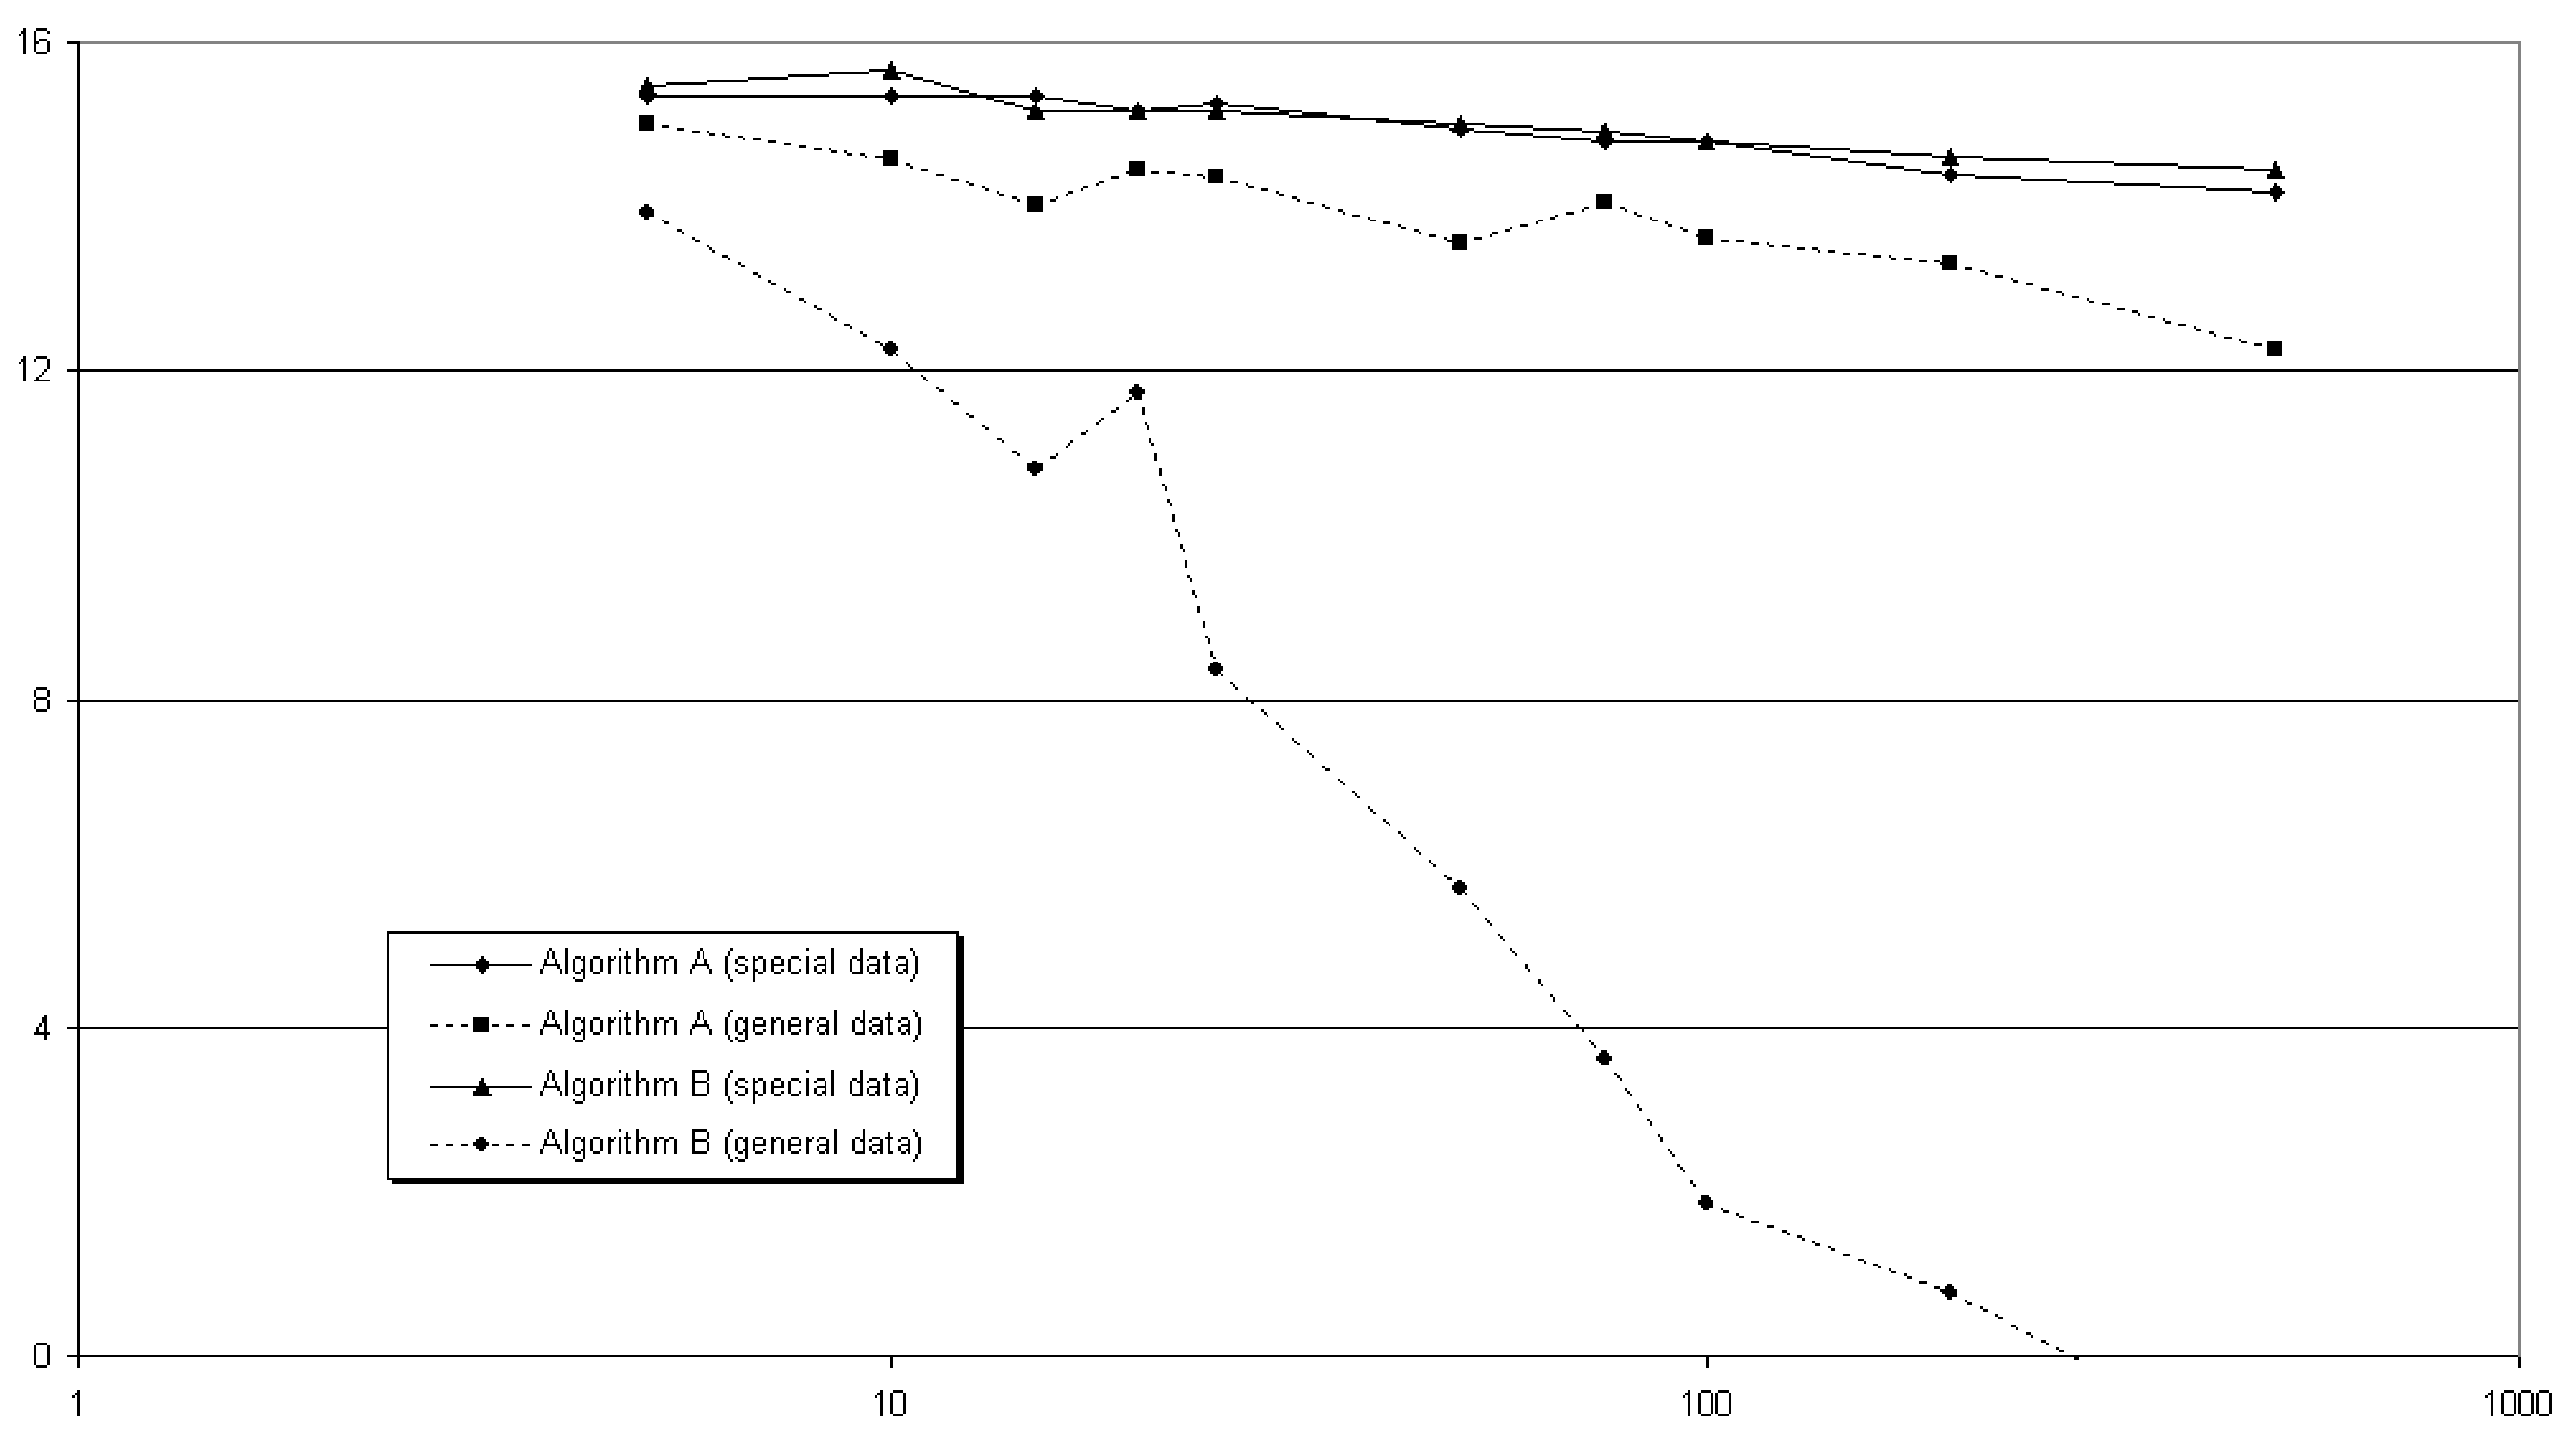
\includegraphics[width=12cm]{Figures/Precision}
\caption{Comparison of achieved precision} \label{fig:precision}
\end{figure}
Figure \ref{fig:precision} shows the results. The parameter
measuring the complexity is laid on the $x$-axis using a
logarithmic scale. The precision is expressed as the negative of
the decimal logarithm of the deviation from the known solution.
The higher the value the better is the precision. The precision of
the floating-point numbers on the machine used in this study
corresponds roughly to 16 on the scale of Figure
\ref{fig:precision}.

The first observation does not come as a surprise: the precision
of each algorithm degrades as the complexity of the problem
increases. One can see that when the algorithms can exploit the
symmetry properties of the data the precision is better (curves
for special data) than for general data. In this case the two
algorithms are performing with essentially the same precision.
Thus, one can chose the faster algorithm, namely algorithm B. For
the general data, however, algorithm B has poorer and poorer
precision as the complexity increases. For complexity larger than
50 algorithm B becomes totally unreliable, to the point of
becoming a perfect illustration of Knuth's quotation above. Thus,
for general data, one has no choice but to use algorithm A.

Readers who do not like mysteries can go read section
\ref{sec:matrixrounding} where these algorithms are discussed.

\subsection{Outsmarting rounding errors}
\label{sec:outsmart} In some instances rounding errors can be
significantly reduced if one spends some time reconsidering how to
compute the final solution. In this section we like to show an
example of such thinking.

Consider the following second order equation, which must be solved
when looking for the eigenvalues of a symmetric matrix (\cf
section \ref{sec:eigensym}):
\begin{equation}
\label{eq:round2nd}
  t^2+2\alpha t - 1 =0.
\end{equation}
Without restricting the generality of the argumentation, we shall
assume that $\alpha$ is positive. the problem is to find the the
root of equation \ref{eq:round2nd} having the smallest absolute
value. You, reader, should have the answer somewhere in one corner
of your brain, left over from high school mathematics:
\begin{equation}
\label{eq:round2ndsol}
  t_{\min}=\sqrt{\alpha^2+1} - \alpha.
\end{equation}
Let us now assume that $\alpha$ is very large, so large that
adding $1$ to $\alpha^2$ cannot be noticed within the machine
precision. Then, the smallest of the solutions of equation
\ref{eq:round2nd} becomes $t_{\min}\approx 0$, which is of course
not true: the left hand side of equation  \ref{eq:round2nd}
evaluates to $-1$.

\noindent Let us now rewrite equation \ref{eq:round2nd} for the
variable $x=1/t$. This gives the following equation:
\begin{equation}
\label{eq:round2ndinv}
  x^2-2\alpha x - 1 =0.
\end{equation}
The smallest of the two solutions of equation \ref{eq:round2nd} is
the largest of the two solutions of equation \ref{eq:round2ndinv}.
That is:
\begin{equation}
  t_{\min}={1\over x_{\max}}={1 \over \sqrt{\alpha^2+1} + \alpha}.
\end{equation}
Now we have for large $\alpha$:
\begin{equation}
  t_{\min}\approx {1\over 2\alpha}.
\end{equation}
This solution has certainly some rounding errors, but much less
than the solution of equation \ref{eq:round2ndsol}: the left hand
side of equation \ref{eq:round2nd} evaluates to ${1\over
4\alpha^2}$, which goes toward zero for large $\alpha$, as it
should be.

\subsection{Wisdom from the past}
To close the subject of rounding errors, I would like to give the
reader a different perspective. There is a big difference between
a full control of rounding errors and giving a result with high
precision. Granted, high precision computation is required to
minimize rounding errors. On the other hand, one only needs to
keep the rounding errors under control to a level up to the
precision required for the final results. There is no need to
determine a result with non-sensical precision.

To illustrate the point, I am going to use a very old mathematical
problem: the determination of the number $\pi$. The story is taken
from the excellent book of Jan Gullberg, {\em Mathematics From the
Birth of the Numbers} \cite{Gullberg}.

Around 300BC, Archimedes devised a simple algorithm to approximate
$\pi$. For a circle of diameter $d$, one computes the perimeter
$p_{\mathop{\rm in}}$ of a $n$-sided regular polygon inscribed
within the circle and the perimeter $p_{\mathop{\rm out}}$ of a
$n$-sided regular polygon whose sides the tangent to the same
circle. We have:
\begin{equation}
{\displaystyle p_{\mathop{\rm in}} \over\displaystyle d
}<\pi<{\displaystyle p_{\mathop{\rm out}} \over\displaystyle d}.
\end{equation}
By increasing $n$, one can improve the precision of the
determination of $\pi$. During the Antiquity and the Middle Age,
the computation of the perimeters was a formidable task and an
informal competition took place to find who could find the most
precise approximation of the number $\pi$. In 1424, Jamshid Masud
al-Kashi, a persian scientist, published an approximation of $\pi$
with 16 decimal digits. The number of sides of the polygons was
$3\times 2^8$. This was quite an achievement, the last of its
kind. After that, mathematicians discovered other means of
expressing the number $\pi$.

In my eyes, however, Jamshid Masud al-Kashi deserves fame and
admiration for the note added to his publication that places his
result in perspective. He noted that the precision of his
determination of the number $\pi$ was such that,
\begin{quote}{\it the error
in computing the perimeter of a circle with a radius 600�000 times
that of earth would be less than the thickness of a horse�s hair}.
\end{quote}
The reader should know that the {\it thickness of a horse�s
hair\/} was a legal unit of measure in ancient Persia
corresponding to roughly 0.7 mm. Using present-day knowledge of
astronomy, the radius of the circle corresponding to the error
quoted by Jamshid Masud al-Kashi is 147 times the distance between
the sun and the earth, or about 3 times the radius of the orbit of
Pluto, the most distant planet of the solar system.

As Jan Gullberg notes in his book, {\it al-Kashi evidently had a
good understanding of the meaninglessness of long chains of
decimals}. When dealing with numerical precision, you should ask
yourself the following question:
\begin{quote}
{\sl Do I really need to know the length of Pluto's orbit to a
third of the thickness of a horse�s hair?}
\end{quote}

\section{Finding the numerical precision of a computer}
\label{sec:findprecision}
Object-oriented languages such as Smalltalk and Java give the
opportunity to develop an application on one hardware platform and
to deploy the application on other platforms running on different
operating systems and hardware. It is a well-known fact that the
marketing about Java was centered about the concept of {\sl Write
Once Run Anywhere}. What fewer people know is that this concept
already existed for Smalltalk 10 years before the advent of Java.

Some numerical algorithms are carried until the estimated
precision of the result becomes smaller than a given value, called
the desired precision. Since an application can be executing on
different hardware, the desired precision is best determined at
run time.

The book of Press {\it et al.} \cite{Press} shows a clever code
determining all the parameters of the floating-point
representation of a particular computer. In this book we shall
concentrate only on the parameters which are relevant for
numerical computations. These parameters correspond to the
instance variables of the object responsible to compute them. They
are the following:
\begin{description}
\item[{\tt radix}] the radix of the floating-point representation, that is $r$.
\item[{\tt machinePrecision}] the largest positive number which, when added to 1 yields 1.
\item[{\tt negativeMachinePrecision}] the largest positive number which, when subtracted from 1 yields 1.
\item[{\tt smallestNumber}] the smallest positive number different from 0.
\item[{\tt largestNumber}] the largest positive number which can be represented in the machine.
\item[{\tt defaultNumericalPrecision}] the relative precision, which can be expected for a general numerical computation.
\item[{\tt smallNumber}] a number, which can be added to some value without noticeably changing the result of the computation.
\end{description}
Computing the radix $r$ is done in two steps. First one computes a
number equivalent of the machine precision (\cf next paragraph)
assuming the radix is 2. Then, one keeps adding 1 to this number
until the result changes. The number of added ones is the radix.

The machine precision is computed by finding the largest integer
$n$ such that:
\begin{equation}
\left(1+r^{-n}\right)-1\ne 0
\end{equation}
This is done with a loop over $n$. The quantity
$\epsilon_+=r^{-\left(n+1\right)}$ is the machine precision.

The negative machine precision is computed by finding the largest
integer $n$ such that:
\begin{equation}
\left(1-r^{-n}\right)-1\ne 0
\end{equation}
Computation is made as for the machine precision. The quantity
$\epsilon_-=r^{-\left(n+1\right)}$ is the negative machine
precision. If the floating-point representation uses
two-complement to represent negative numbers the machine precision
is larger than the negative machine precision.

To compute the smallest and largest number one first compute a
number whose mantissa is full. Such a number is obtained by
building the expression $f=1-r \times \epsilon_-$. The smallest
number is then computed by repeatedly dividing this value by the
radix until the result produces an underflow. The last value
obtained before an underflow occurs is the smallest number.
Similarly, the largest number is computed by repeatedly
multiplying the value $f$ until an overflow occurs. The last value
obtained before an overflow occurs is the largest number.

The variable {\tt defaultNumericalPrecision} contains an estimate
of the precision expected for a general numerical computation. For
example, one should consider that two numbers $a$ and $b$ are
equal if the relative difference between them is less than the
default numerical machine precision. This value of the default
numerical machine precision has been defined as the square root of
the machine precision.

The variable {\tt smallNumber} contains a value, which can be
added to some number without noticeably changing the result of the
computation. In general an expression of the type $0 \over 0$ is
undefined. In some particular case, however, one can define a
value based on a limit. For example, the expression $\sin x \over
x $ is equal to 1 for $x=0$. For algorithms, where such an
undefined expression can occur\footnote{Of course, after making
sure that the ratio is well defined numerically.}, adding a small
number to the numerator and the denominator can avoid the division
by zero exception and can obtain the correct value. This value of
the small number has been defined as the square root of the
smallest number that can be represented on the machine.

\subsection{Computer numerical precision}
The computation of the parameters only needs to be executed once.
We have introduced a specific class to hold the variables
described earlier and made them available to any object.

Each parameter is computed using lazy initialization within the
method bearing the same name as the parameter. Lazy initialization
is used while all parameters may not be needed at a given time.
Methods in charge of computing the parameters are all prefixed
with the word compute.

Listing \ref{ls:floatmachine} shows the class {\tt
DhbFloatingPointMachine} responsible of computing the parameters
of the floating-point representation. This class is implemented as
a singleton class because the parameters need to be computed once
only. For that reason no code optimization was made and priority
is given to readability.

\noindent The computation of the smallest and largest numbers uses
exceptions to detect the underflow and the overflow.

\noindent The method {\tt showParameters} can be used to print the
values of the parameters onto the Transcript window.

\begin{listing} Smalltalk code to find the machine precision
  \label{ls:floatmachine}
  $$\halign{ #\hfil&\quad#\hfil\cr {\sl Class}& {\Large\bf DhbFloatingPointMachine}\cr
{\sl Subclass of }&{\tt Object}\cr\noalign{\vskip 1ex}

{\sl Instance variable names:}&\parbox[t]{4 in}{\tt  defaultNumericalPrecision radix machinePrecision negativeMachinePrecision smallestNumber largestNumber smallNumber largestExponentArgument }\cr\noalign{\vskip 1ex}
{\sl Class variable names:}&\parbox[t]{4 in}{\tt  UniqueInstance }\cr\noalign{\vskip 1ex}}$$


Class methods
{\parskip 1ex\par\noindent}
{\bf new}
\begin{verbatim}
    UniqueInstance = nil
        ifTrue: [ UniqueInstance := super new].
    ^UniqueInstance

\end{verbatim}
{\bf reset}
\begin{verbatim}
    UniqueInstance := nil.

\end{verbatim}



Instance methods
{\parskip 1ex\par\noindent}
{\bf computeLargestNumber}
\begin{verbatim}
    | zero one floatingRadix fullMantissaNumber |
    zero := 0 asFloat.
    one := 1 asFloat.
    floatingRadix := self radix asFloat.
    fullMantissaNumber := one - ( floatingRadix * self 
                                            negativeMachinePrecision).
    largestNumber := fullMantissaNumber.
    [ [ fullMantissaNumber := fullMantissaNumber * floatingRadix.
        largestNumber := fullMantissaNumber.
        true] whileTrue: [ ].
        ] when: ExAll do: [ :signal | signal exitWith: nil].

\end{verbatim}
{\bf computeMachinePrecision}
\begin{verbatim}
    | one zero a b inverseRadix tmp x |
    one := 1 asFloat.
    zero := 0 asFloat.
    inverseRadix := one / self radix asFloat.
    machinePrecision := one.
    [ tmp := one + machinePrecision.
      tmp - one = zero]
        whileFalse:[  machinePrecision := machinePrecision * 
                                                        inverseRadix].

\end{verbatim}
{\bf computeNegativeMachinePrecision}
\begin{verbatim}
    | one zero floatingRadix inverseRadix tmp |
    one := 1 asFloat.
    zero := 0 asFloat.
    floatingRadix := self radix asFloat.
    inverseRadix := one / floatingRadix.
    negativeMachinePrecision := one.
    [ tmp := one - negativeMachinePrecision.
      tmp - one = zero]
        whileFalse:[ negativeMachinePrecision := 
                             negativeMachinePrecision * inverseRadix].

\end{verbatim}
{\bf computeRadix}
\begin{verbatim}
    | one zero a b tmp1 tmp2|
    one := 1 asFloat.
    zero := 0 asFloat.
    a := one.
    [ a := a + a.
      tmp1 := a + one.
      tmp2 := tmp1 - a.
      tmp2 - one = zero] whileTrue:[].
    b := one.
    [ b := b + b.
      tmp1 := a + b.
      radix := ( tmp1 - a) truncated.
      radix = 0 ] whileTrue: [].

\end{verbatim}
{\bf computeSmallestNumber}
\begin{verbatim}
    | zero one floatingRadix inverseRadix fullMantissaNumber |
    zero := 0 asFloat.
    one := 1 asFloat.
    floatingRadix := self radix asFloat.
    inverseRadix := one / floatingRadix.
    fullMantissaNumber := one - ( floatingRadix * self 
                                            negativeMachinePrecision).
    smallestNumber := fullMantissaNumber.
    [ [ fullMantissaNumber := fullMantissaNumber * inverseRadix.
        smallestNumber := fullMantissaNumber.
        true] whileTrue: [ ].
        ] when: ExAll do: [ :signal | signal exitWith: nil].

\end{verbatim}
{\bf defaultNumericalPrecision}
\begin{verbatim}
    defaultNumericalPrecision isNil
        ifTrue: [ defaultNumericalPrecision := self machinePrecision 
                                                                sqrt].
    ^defaultNumericalPrecision

\end{verbatim}
{\bf largestExponentArgument}
\begin{verbatim}
    largestExponentArgument isNil
        ifTrue: [ largestExponentArgument := self largestNumber ln].
    ^largestExponentArgument

\end{verbatim}
{\bf largestNumber}
\begin{verbatim}
    largestNumber isNil
        ifTrue: [ self computeLargestNumber].
    ^largestNumber

\end{verbatim}
{\bf machinePrecision}
\begin{verbatim}
    machinePrecision isNil
        ifTrue: [ self computeMachinePrecision].
    ^machinePrecision

\end{verbatim}
{\bf negativeMachinePrecision}
\begin{verbatim}
    negativeMachinePrecision isNil
        ifTrue: [ self computeNegativeMachinePrecision].
    ^negativeMachinePrecision

\end{verbatim}
{\bf radix}
\begin{verbatim}
    radix isNil
        ifTrue: [ self computeRadix].
    ^radix

\end{verbatim}
{\bf showParameters}
\begin{verbatim}
    Transcript cr; cr;
            nextPutAll: 'Floating-point machine parameters'; cr;
            nextPutAll: '---------------------------------';cr;
            nextPutAll: 'Radix: '.
    self radix printOn: Transcript.
    Transcript cr; nextPutAll: 'Machine precision: '.
    self machinePrecision printOn: Transcript.
    Transcript cr; nextPutAll: 'Negative machine precision: '.
    self negativeMachinePrecision printOn: Transcript.
    Transcript cr; nextPutAll: 'Smallest number: '.
    self smallestNumber printOn: Transcript.
    Transcript cr; nextPutAll: 'Largest number: '.
    self largestNumber printOn: Transcript.         

\end{verbatim}
{\bf smallestNumber}
\begin{verbatim}
    smallestNumber isNil
        ifTrue: [ self computeSmallestNumber].
    ^smallestNumber

\end{verbatim}
{\bf smallNumber}
\begin{verbatim}
    smallNumber isNil
        ifTrue: [ smallNumber := self smallestNumber sqrt].
    ^smallNumber

\end{verbatim}


\end{listing}


\section{Comparing floating point numbers}
It is very surprising to see how frequently questions about the
lack of equality between two floating-point numbers are posted on
the Smalltalk electronic discussion groups. As we have
seen in section \ref{sec-rounding} one should always expect the
result of two different computations that should have yielded the
same number from a mathematical standpoint to be different using a
finite  numerical representation. Somehow the computer courses are
not giving enough emphasis about floating-point numbers.

\begin{quote}
So, how should you check the equality of two floating-point
numbers? \linebreak\noindent\hfil The practical answer is: {\sl
thou shalt not!}
\end{quote}

\noindent As you will see, the algorithms in this book only
compare numbers, but never check for equality. If you cannot
escape the need for a test of equality, however, the best solution
is to create methods to do this. Since the floating-point
representation is keeping a constant relative precision,
comparison must be made using relative error. Let $a$ and $b$ be
the two numbers to be compared. One should build the following
expression:
\begin{equation}
\label{eq:relerror}
\epsilon={\left|a-b\right| \over
\max\left(\left|a\right|,\left|b\right|\right)}
\end{equation}
The two numbers can be considered equal if $\epsilon$ is smaller
than a given number $\epsilon_{\max}$. If the denominator of the
fraction on equation \ref{eq:relerror} is less than
$\epsilon_{\max}$, than the two numbers can be considered as being
equal. For lack of information on how the numbers $a$ and $b$ have
been obtained, one uses for $\epsilon_{\max}$ the default
numerical precision defined in section \ref{sec:findprecision}. If
one can determine the precision of each number, then the method
{\tt relativelyEqual} can be used.

In Smalltalk this means adding a new method to the class Number as
shown in Listing \ref{ls:fltcompare}.

\begin{listing}
Comparison of floating point numbers in Smalltalk
\label{ls:fltcompare}
$$\halign{ #\hfil&\quad#\hfil\cr {\sl Class}& {\Large\bf Number}\cr
{\sl Subclass of }&{\tt Magnitude}\cr\noalign{\vskip 1ex}
}$$


Instance methods
{\parskip 1ex\par\noindent}
{\bf equalsTo:} {\tt aNumber}
\begin{verbatim}
    ^self relativelyEqualsTo: aNumber 
          upTo: DhbFloatingPointMachine new defaultNumericalPrecision
\end{verbatim}
{\bf relativelyEqualsTo:} {\tt aNumber} {\bf upTo:} {\tt aSmallNumber}
\begin{verbatim}
    | norm |
    norm := self abs max: aNumber abs.
    ^ norm <= DhbFloatingPointMachine new defaultNumericalPrecision
        or: [ (self - aNumber) abs < ( aSmallNumber * norm)]
\end{verbatim}


\end{listing}

\section{Speed consideration (to be revisited)}
\label{sec:speed} Some people may think that implementing
numerical methods for object-oriented languages such as Smalltalk just a waste
of time. Those languages are notoriously slow or so they think.

First of all, things should be put in perspective with other
actions performed by the computer. If a computation does not take
longer than the time needed to refresh a screen, it does not
really matter if the application is interactive. For example,
performing a least square fit to a histogram in Smalltalk and drawing the
resulting fitted function is usually hardly perceptible to the eye on a personal
computer. Thus, even though a C version runs 10 times faster, it
does not make any difference for the end user. The main difference
comes, however, when you need to modify the code. Object-oriented
software is well known for its maintainability. As $80\%$ of the
code development is spent in maintenance this aspect should first
be considered.

Table \ref{tb:speed} shows measured speed of execution for some of
the algorithms exposed in this book. Timing was done on a personal
computer equipped with a Pentium II clocked at 200MHz and running
Windows NT workstation 4.0. The C code used is the code of
\cite{Press} compiled with the C compiler Visual C$^{++}$ 4.0 from
Microsoft Corporation. The time needed to allocate memory for
intermediate results was included in the measurement of the C
code, otherwise the comparison with object-oriented code would not
be fair. The Smalltalk code was run under version 4.0 of Visual
Age\tm for Smalltalk from IBM Corporation using the ENVY benchmark
tool provided.
Elapsed time were measured
by repeating the measured evaluation a sufficient number of time
so that the error caused by the CPU clock is less that the last
digit shown in the final result.
\begin{table}[h]
\caption{Compared execution speed between C and Smalltalk}
\label{tb:speed} \vspace{1 ex}
\begin{tabular}{|l | c r r |} \hline
  \hfil {\bf Operation} & {\bf Units} & {\bf C}\hfil & {\bf Smalltalk}\hfil \\ \hline
  Polynomial $10\th$ degree & msec. & 1.1 & 27.7 \\
  Neville interpolation (20 points) & msec. & 0.9 & 11.0 \\
  LUP matrix inversion ($100\times 100$)& sec. & 3.9 & 22.9 \\ \hline
\end{tabular}
\end{table}

One can see that object-oriented code is quite efficient,
especially when it comes to complex algorithms: good
object-oriented code can actually beat up C code.

%My early tests with Java, a couple of years ago, were showing that
%Java was 5-10 times slower than C. One can see that vendors did a
%great job in optimizing the generated code and in accelerating the
%virtual machine. I would like to see the same efforts going in
%optimizing Smalltalk. The spectacular improvement of Java shows
%that it is possible. Actually, my early tests made with Visual
%Smalltalk\tm from Digitalk Inc.\footnote{Unfortunately, the future
%of Visual Smalltalk now owned by Cincom Inc. is quite uncertain at
%this time of writing.} were 5 times better.

%Today admittedly, I would not use Smalltalk to build a structural
%analysis program, but Java would certainly be a contender.
I have successfully build data mining Smalltalk
applications using {\bf all the code}\footnote{I want to emphasize
here that all the code of this book is real code, which I have
used personally in real applications.} presented in this book.
These applications were not perceived as slow by the end user
since most of the computer time was spent drawing the data.

\subsection{Smalltalk particular}
Smalltalk has an interesting property: a division between two
integers is by default kept as a fraction. This prevents rounding
errors. For example, the multiplication of a matrix of integer
numbers with its inverse always yields an exact identity matrix.
(\cf section \ref{sec:lup} for definitions of these terms).

There is, however, a price to pay for the perfection offered by
fractions. When using fractions, the computing time often becomes
prohibitive. Resulting fractions are often composed of large
integers. This slows down the computing. In the case of matrix
inversion, this results in an increase in computing time by
several orders of magnitude.

For example, one of my customers was inverting a $301\times 301$
matrix with the code of section \ref{sec:lup}. The numbers used to
build the matrix where obtained from a measuring device (using an
ADC) and where thus integers. The inversion time was over 2
hours\footnote{This particular customer was a {\sl very} patient
person!}. After converting the matrix components to floating
numbers the inversion time became less than 30 seconds!

If you are especially unlucky you may run out of memory when
attempting to store a particularly long integer. Thus, it is
always a good idea to use floating\footnote{In most available
Smalltalk versions the class Float corresponds to floating numbers
with double precision. VisualWorks makes the difference between
{\tt Float} and {\tt Double}} numbers instead of fractions unless
absolute accuracy is your primary goal. My experience has been
that using floating numbers speeds up the computation by at least
an order of magnitude. In the case of complex computations such as
matrix inversion or least square fit this can become prohibitive.

\section{Conventions}
Equations presented in this book are using standard international
mathematical notation as described in \cite{Knuth1}. Each section
is trying to made a quick derivation of the concepts needed to
fully understand the mathematics behind the scene. For readers in
a hurry, the equations used by the implementation are flagged as
the following sample equation:
\begin{mainEquation}
\ln ab = \ln a + \ln b.
\end{mainEquation}
When such an equation is encountered, the reader is sure that the
expression is implemented in the code.

In general the code presented in this book adheres to conventions
widely used in each language. Having said that, there are a few
instances where we have departed from the widely used conventions.

\subsection{Class diagrams}
When appropriate a class diagram is shown at the beginning of each
chapter. This diagram shows the hierarchy of the classes described
in the chapter and eventually the relations with classes of other
chapters. The diagrams are drawn using the conventions of the book
on design patterns \cite{GoF}.

Figure \ref{fig:classDiagram} shows a typical class diagram. A
rectangular box with 2 or 3 parts represents a class. The top part
contains the name of the class in bold face. If the class is an
abstract class the name in shown in italic bold face. In figure
\ref{fig:classDiagram} the classes {\tt RelatedClass}, {\tt
MySubClass1} and {\tt MySubclass2} are concrete classes; {\tt
MyAbstractClass} is an abstract class. The second part of the
class box contains a list of the public instance methods. The name
of an abstract method is written in italic, for example {\tt
abstractMethod3} in the class {\tt MyAbstractClass} of figure
\ref{fig:classDiagram}. The third part of the class box, if any,
contains the list of all instance variables. If the class does not
have any instance variable the class box only consists of 2 parts,
for example the class {\tt MySubClass1} of figure
\ref{fig:classDiagram}.
\begin{figure}
\centering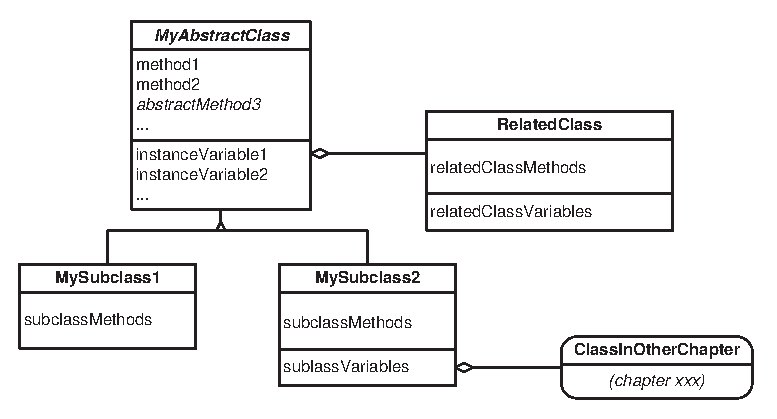
\includegraphics[width=11cm]{Figures/TypicalClassDiagram}
\caption{A typical class diagram} \label{fig:classDiagram}
\end{figure}

A vertical line with a triangle indicates class inheritance. If
there are several subclasses the line branches at the triangle, as
this is the case in figure \ref{fig:classDiagram}. A horizontal
line beginning with a diamond (UML aggregation symbol) indicates
the class of an instance variable. For example, Figure
\ref{fig:classDiagram} indicates that the instance variable {\tt
instanceVariable1} of the class {\tt MyAbstractClass} must be an
instance of the class {\tt RelatedClass}. The diamond is black is
the instance variable is a collection of instances of the class. A
class within a rectangle with rounded corner represents a class
already discussed in an earlier chapter; the reference to the
chapter is written below the class name. Class {\tt
ClassInOtherChapter} in figure \ref{fig:classDiagram} is such a
class. To save space, we have used the
Smalltalk method names. It is quite easy to identify methods
needing parameters when one uses Smalltalk method names: a
colon in the middle or at the end of the method name indicates
a parameter. Please refer to appendix \ref{ch:smalltalkprimer} for
more details on Smalltalk methods.

\subsection{Smalltalk code}
Most of the Smalltalk systems do not support name spaces. As a
consequence, it has becomed a convention to prefix all class names
with 3-letter code identifying the origin of the code. In this
book the names of the Smalltalk classes are all prefixed with the
author's initials.

There are several ways to store constants needed by all instances
of a class. One way is to store the constants in class variables.
This requires each class to implement an initialization method,
which sets the desired values into the class variables. Another
way is to store the constants in a pool dictionary. Here also an
initialization method is required. In my opinion pool dictionaries
are best used for texts, as they provide a convenient way to
change all text from one language to another. Sometimes the
creation of a singleton object is used. This is especially useful
when the constants are installation specific and, therefore, must
be determined at the beginning of the application's execution,
such as the precision of the machine (\cf section
\ref{sec:findprecision}). Finally constants which are not likely
to change can be stored in the code. This is acceptable as long as
this is done at a unique place. In this book most constants are
defined in class methods.

By default a Smalltalk method returns {\tt self}. For
initialization methods, however, we write this return explicitly
({\tt \^\/self}) to ease reading. This adheres to the intention
revealing patterns of Kent Beck \cite{Beck}.

In \cite{StDesPat} it is recommended to use the method name {\tt
default} to implement a singleton class. In this book this
convention is not followed. In Smalltalk, however, the normal
instance creation method is {\tt new}. Introducing a method {\tt
default} for singleton classes has the effect of departing from
this more ancient convention. In fact, requiring the use of {\tt
default} amounts to reveal to the client the details of
implementation used by the class. This is in clear contradiction
with the principle of hiding the implementation to the external
world. Thus, singleton classes in all code presented in this book
are obtained by sending the method {\tt new} to the class. A
method named {\tt default} is reserved for the very semantic of
the word default: the instance returned by these methods is an
instance initialized with some default contents, well specified.
Whether or not the instance is a singleton is not the problem of
the client application.



\section{Road map}
This last section of the introduction describes the road map of
the algorithms discussed in the book chapter by chapter. Figure
\ref{fig:roadmap} shows a schematic view of the major classes
discussed in this book together with their dependency relations.
\begin{figure}
\centering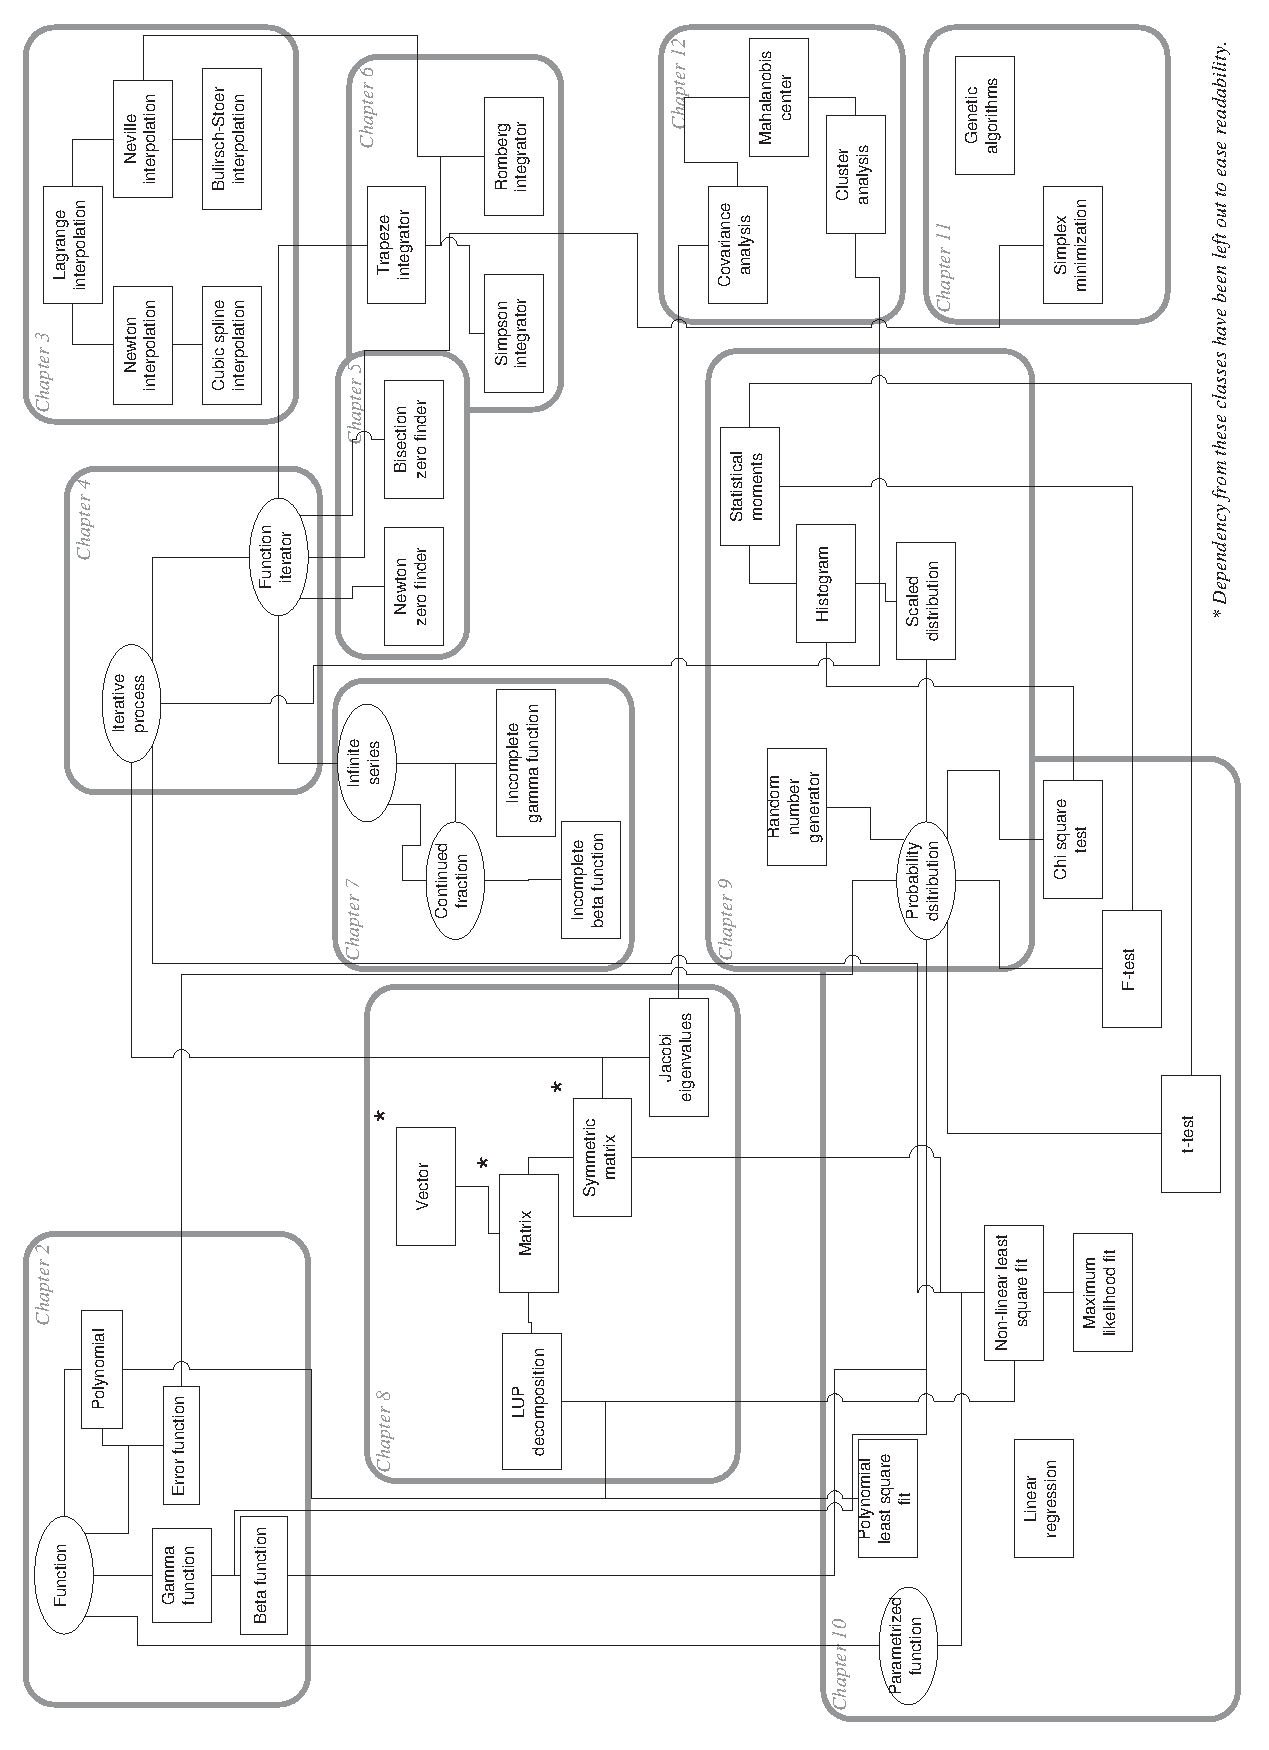
\includegraphics[width=13cm]{Figures/Roadmap}
\caption{Book road map} \label{fig:roadmap}
\end{figure}
In this figure, abstract classes are represented with an ellipse,
concrete classes with a rectangle. Dependencies between the
classes are represented by lines going from one class to another;
the dependent class is always located below. Chapters where the
classes are discussed are drawn as grayed rectangles with rounded
corners. Hopefully the reader will not be scared by the complexity
of the figure. Actually, the figure should be more complex as the
classes {\tt Vector} and {\tt Matrix} are used by most objects
located in chapters \ref{ch:linearalgebra} and following. To
preserve the readability of figure \ref{fig:roadmap} the
dependency connections for these two classes have been left out.

Chapter \ref{ch:function} presents a general representation of
mathematical functions. Examples are shown. A concrete
implementation of polynomial is discussed. Finally three library
functions are given: the error function, the gamma function and
the beta function.

Chapter \ref{ch:interpolation} discusses interpolation algorithms.
A discussion explains when interpolation should be used and which
algorithm is more appropriate to which data.

Chapter \ref{ch:iteration} presents a general framework for
iterative process. It also discusses a specialization of the
framework to iterative process with a single numerical result.
This framework is widely used in the rest of the book.

Chapter \ref{ch:zeroes} discusses two algorithms to find the
zeroes of a function: bisection and Newton's zero finding
algorithms. Both algorithms use the general framework of chapter
\ref{ch:iteration}.

Chapter \ref{ch:integration} discusses several algorithms to
compute the integral of a function. All algorithms are based on
the general framework of chapter \ref{ch:iteration}. This chapter
also uses an interpolation technique from chapter
\ref{ch:interpolation}.

Chapter \ref{ch:series} discusses the specialization of the
general framework of chapter \ref{ch:iteration} to the computation
of infinite series and continued fractions. The incomplete gamma
function and incomplete beta function are used as concrete
examples to illustrate the technique.

Chapter \ref{ch:linearalgebra} presents a concrete implementation
of vector and matrix algebra. It also discusses algorithms to
solve systems of linear equations. Algorithms to compute matrix
inversion and the finding of eigenvalues and eigenvectors are
exposed. Elements of this chapter are used in other part of this
book.

Chapter \ref{ch:statistics} presents tools to perform statistical
analysis. Random number generators are discussed. We give an
abstract implementation of a probability distribution with
concrete example of the most important distributions. The
implementation of other distributions is given in appendix. This
chapter uses techniques from chapters \ref{ch:function},
\ref{ch:zeroes} and \ref{ch:integration}.

Chapter \ref{ch:estimation} discussed the test of hypothesis and
estimation. It gives an implementation of the t- and F-tests. It
presents a general framework to implement least square fit and
maximum likelihood estimation. Concrete implementations of least
square fit for linear and polynomial dependence are given. A
concrete implementation of the maximum likelihood estimation is
given to fit a probability distribution to a histogram. This
chapter uses techniques from chapter \ref{ch:function},
\ref{ch:iteration}, \ref{ch:linearalgebra} and
\ref{ch:statistics}.

Chapter \ref{ch:minimization} discusses some techniques used to
maximize or minimize a function: classical algorithms (simplex,
hill climbing) as well as new ones (genetic algorithms). All these
algorithms are using the general framework for iterative process
discussed in chapter \ref{ch:iteration}.

Chapter \ref{ch:datamining} discusses the modern data mining
techniques: correlation analysis, cluster analysis and neural
networks. A couple of methods invented by the author are also
discussed. This chapter uses directly or indirectly techniques
from all chapters of this book.

\ifx\wholebook\relax\else\end{document}\fi
